\section{GraphMAE原始算法复现}\label{sec:reproduction}
\subsection{五种子结果与训练过程}
表\ref{tab:m1}保留五次正式运行的全部结果。每次均完成1500轮预训练、七次周期Probe和300轮最终Probe，没有提前停止。选中轮次只指最终分类器的验证最优轮次，例如seed4选择第25轮，并不表示只训练了25轮。
\begin{table}[tbp]
\centering\small
\caption{M1原始GraphMAE复现。Accuracy单位为\%，时间为独立worker总耗时，包含导入、数据加载、全部训练/Probe及保存。}\label{tab:m1}
\begin{tabular}{rrrrr}\toprule
Seed & 最佳验证Accuracy & 分类器选中轮次 & 测试Accuracy & 时间/s\\\midrule
0 & 79.80 & 300 & 84.40 & 27.082\\
1 & 79.60 & 300 & 84.50 & 26.497\\
2 & 80.40 & 193 & 83.90 & 25.738\\
3 & 80.60 & 153 & 84.90 & 25.312\\
4 & 80.00 & 25 & 82.20 & 25.832\\\midrule
均值 & 80.08 & --- & 83.98 & 26.092\\\bottomrule
\end{tabular}
\end{table}

图\ref{fig:m1-loss}显示SCE由接近1的初始水平下降，并逐渐进入约0.4量级的波动区间。训练中每轮重新抽取掩码且使用Dropout，故局部起伏并不意味着训练中断。五次训练Loss均为有限值，日志、有效配置、每轮学习率、最佳分类器及最终预训练权重均保留。损失曲线表明重建任务得到优化，但分类表现仍须通过冻结表示的Probe判断。
\begin{figure}[tbp]
\centering
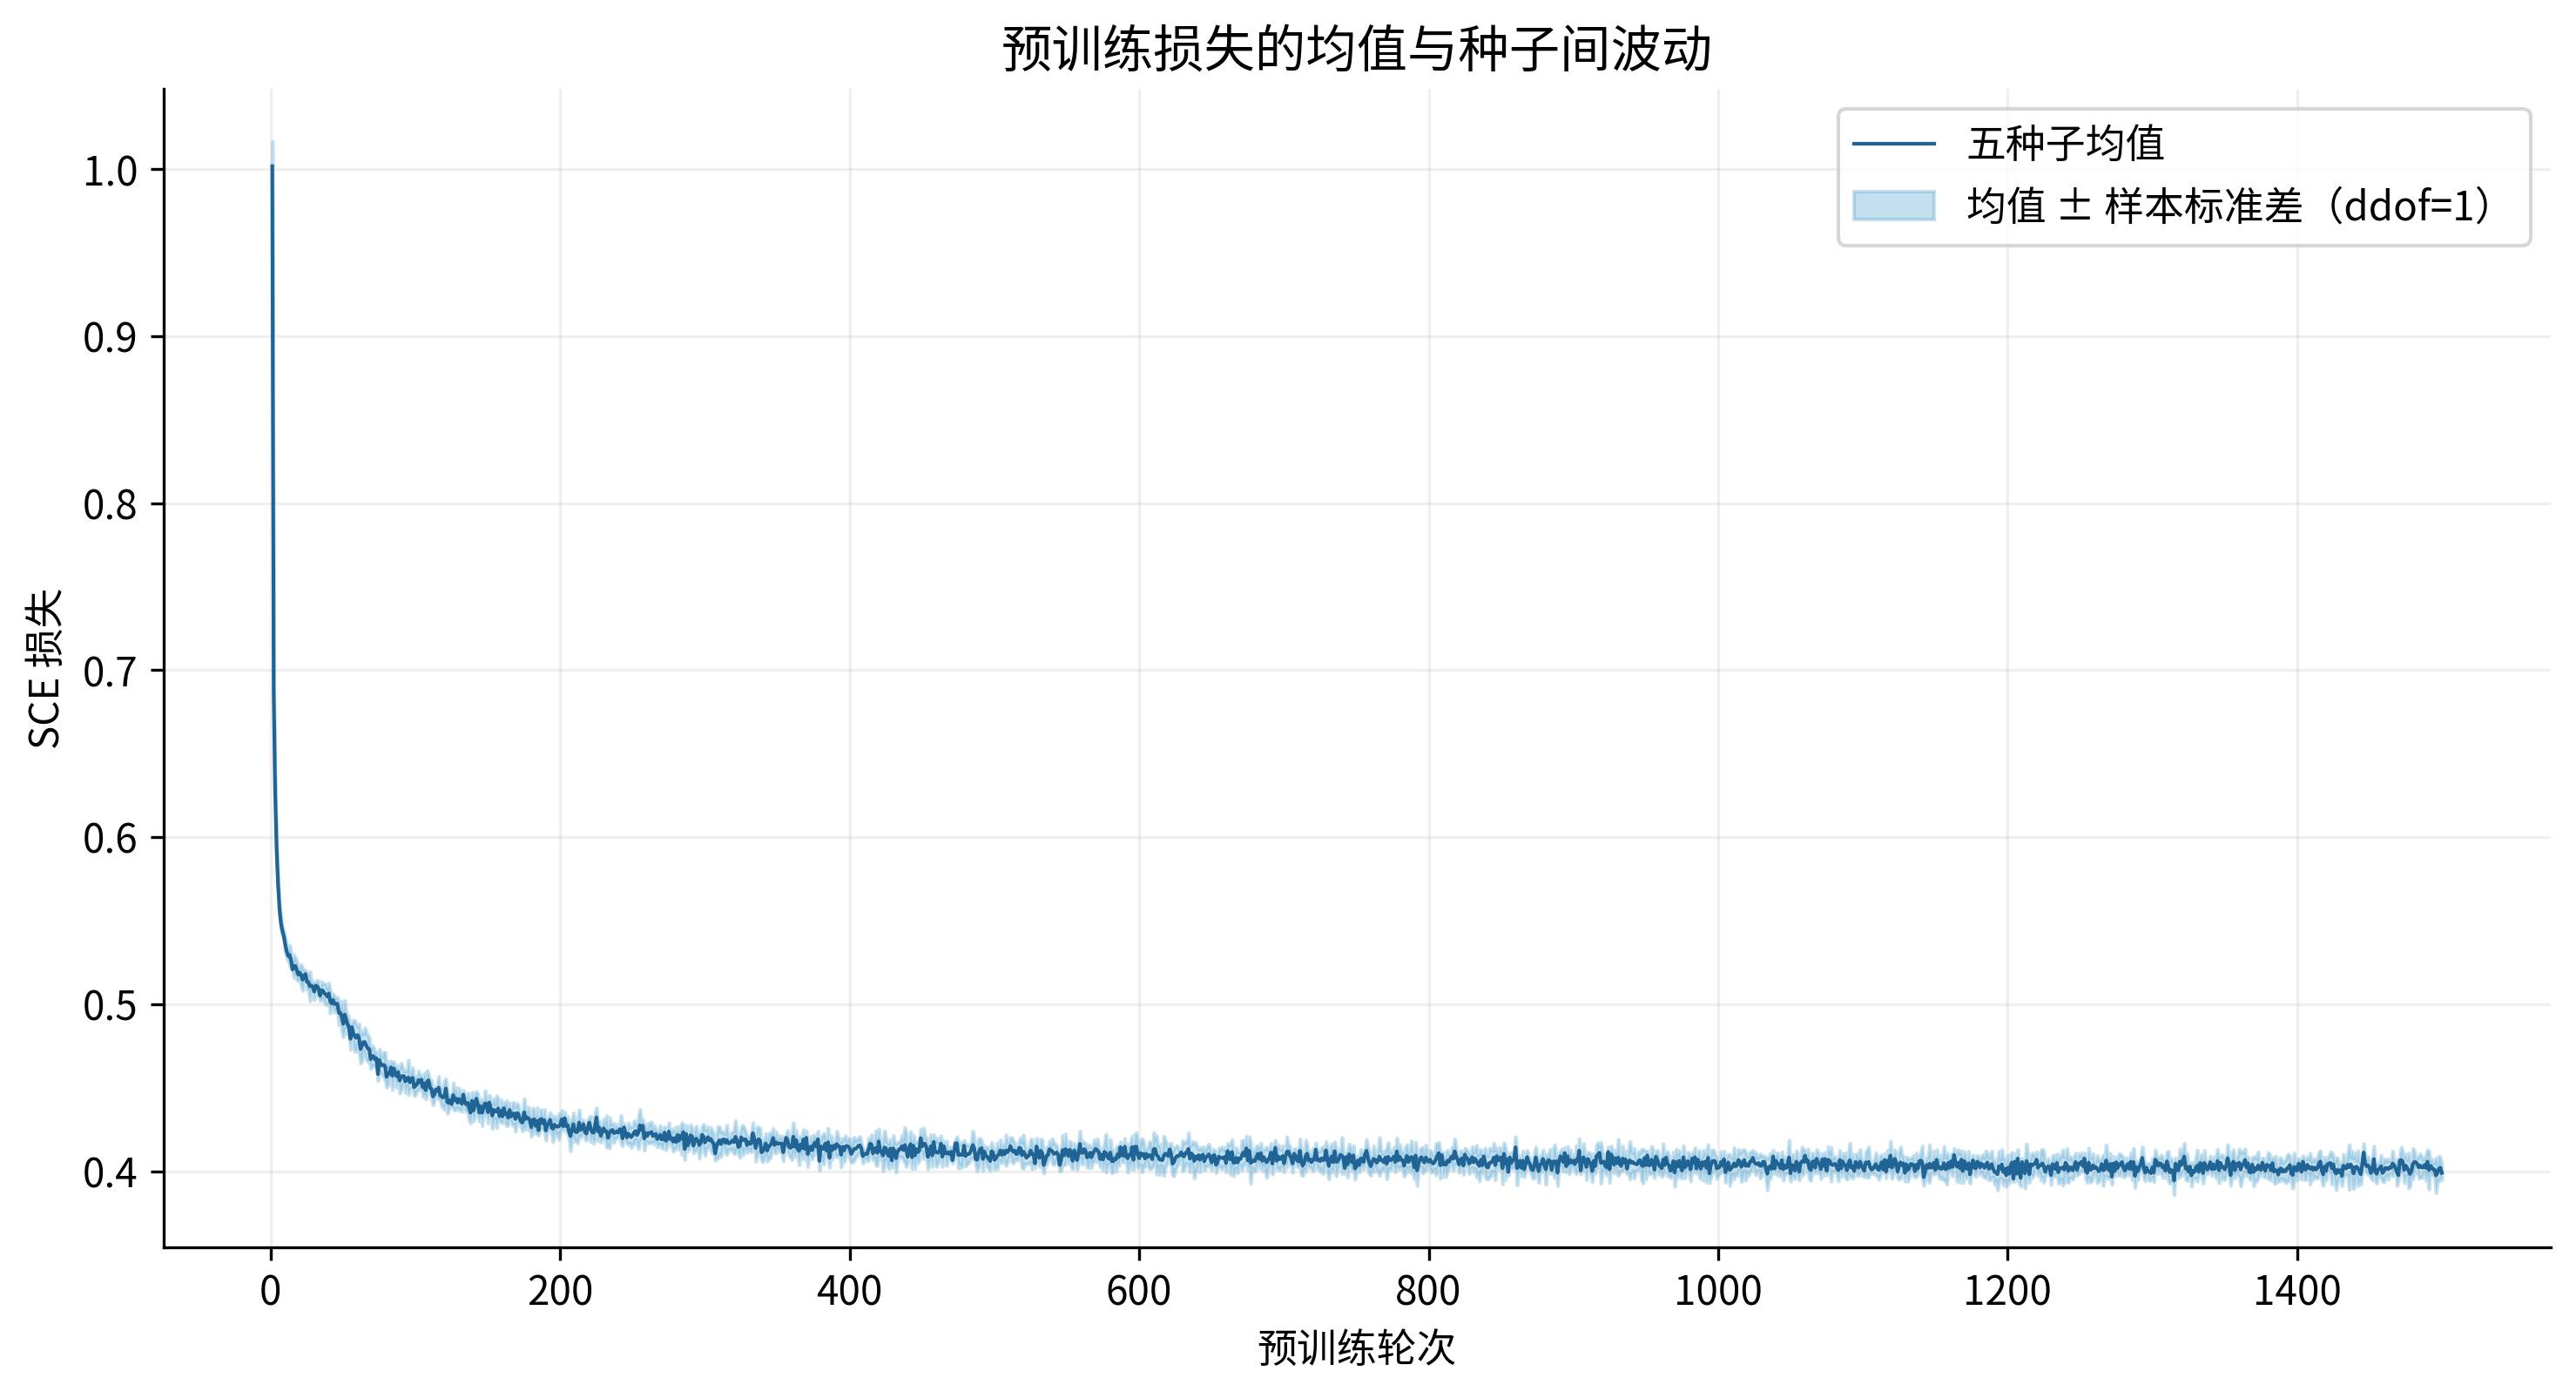
\includegraphics[width=0.86\linewidth]{../figures/M1/loss_mean_std.png}
\caption{M1五种子的预训练SCE均值与波动带。阴影为逐轮跨种子的样本标准差，来源为各次1500轮训练日志；未包含M0短测。}\label{fig:m1-loss}
\end{figure}

\subsection{与原论文结果的参考性比较}
M1测试均值为83.98\%，样本标准差为1.056882个百分点。原论文表1的Cora结果为$84.2\%\pm0.4\%$，采用20次初始化；本项目均值低0.22个百分点。图\ref{fig:m1-accuracy}仅以论文均值提供参考，不代表二者采用完全相同的重复次数和运行环境。
\begin{figure}[tbp]
\centering
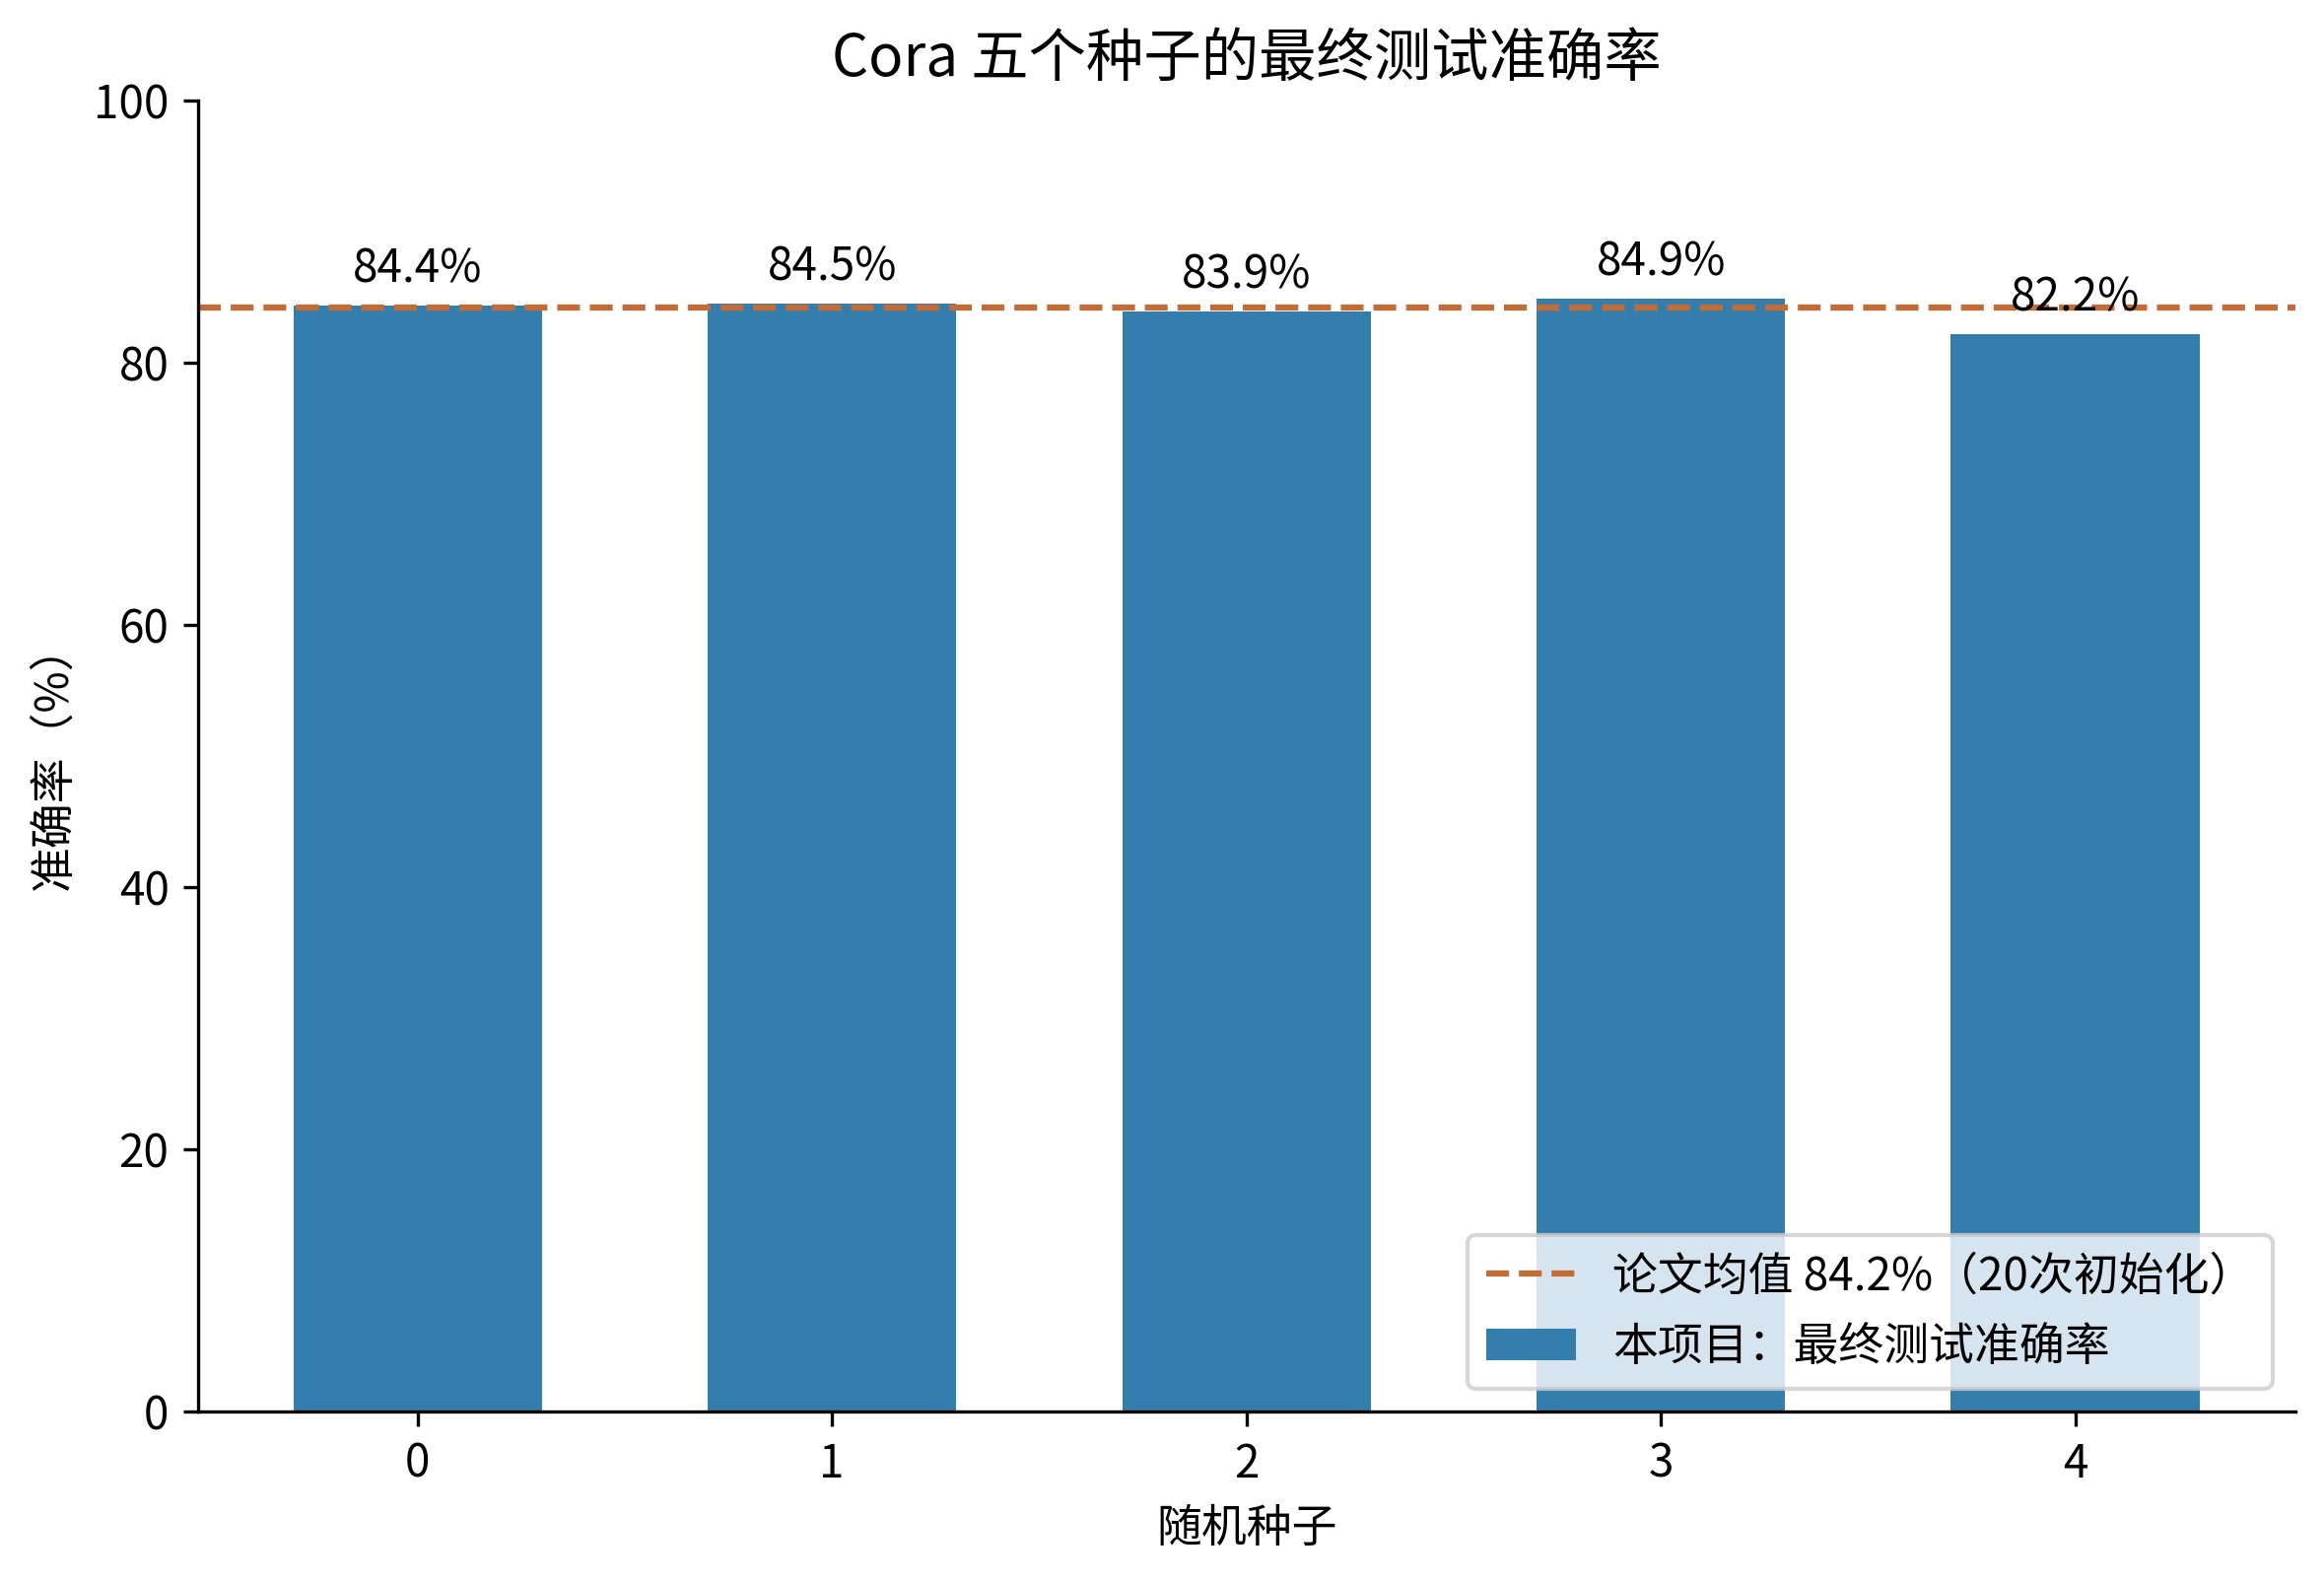
\includegraphics[width=0.86\linewidth]{../figures/M1/accuracy_comparison.png}
\caption{M1五种子的最终测试准确率。虚线为原论文20次初始化的均值84.2\%\cite{hou2022graphmae}；五个柱为本地实测，不能将论文参考线当成本地额外实验。}\label{fig:m1-accuracy}
\end{figure}

五种子的最高与最低准确率为84.9\%和82.2\%，范围为2.7个百分点。seed4虽使总体波动增大，仍按预设种子完整保留，没有重训或剔除。验证最优轮次差异也提示，在只有140个训练标签时，分类器选择对初始化与表示差异较敏感；这是一种现象描述，不足以确定波动来自哪个模型组件。

本次采用PyG、PyTorch 2.4.1和A40，原论文主要使用DGL、PyTorch 1.9和2080Ti。本文使用样本SD，官方代码汇总中\texttt{np.std}默认采用总体SD；原论文未明确给出其标准差实现细节，不能把二者强行视为同一统计口径。此外，本项目仅完成Cora的五次初始化，并未复现其他任务。因此，结果说明锁定官方路径获得了接近论文报告量级的分类表现，同时保留了较大种子波动；不能据均值接近宣称完整复现。
